\section{INTRODUÇÃO}

O marketing digital é uma atividade estratégica para organizações que desejam divulgar produtos e serviços, alcançar públicos específicos e acompanhar resultados por indicadores mensuráveis. Em agências e consultorias, a gestão de tráfego pago envolve a criação e a alteração contínua de campanhas, públicos, orçamentos, criativos e metas em plataformas como Google Ads e Meta Ads. Como diferentes clientes podem demandar essas ações ao mesmo tempo, o trabalho exige coordenação entre atendimento, gestão de tráfego, criação, análise e o próprio cliente.

Entretanto, pedidos de alteração de campanha, aprovação de criativo, envio de relatório e análise de métricas são frequentemente enviados por WhatsApp, e-mail ou mensagens diretas. Esses canais favorecem respostas rápidas, mas dispersam informações e dificultam a identificação do pedido original, a definição de responsável, o acompanhamento de prazo, o registro de aprovação e a recuperação das decisões tomadas. O resultado pode ser retrabalho, atrasos, perda de contexto e baixa transparência no atendimento.

Estudos sobre agências de marketing digital apontam planejamento, comunicação, monitoramento, controle, gestão de tempo e análise de dados como competências necessárias à condução de projetos \cite{steponaitis2023}. Por sua vez, plataformas integradas de automação evidenciam o valor de concentrar atividades, indicadores e responsabilidades em um mesmo ambiente \cite{gujar2024,younas2025}. Nesse cenário, este trabalho propõe o SIGE Desk: uma aplicação web de Help Desk para centralizar e rastrear demandas de tráfego pago.

O sistema será voltado ao registro, à triagem, à atribuição, ao acompanhamento, à validação e ao encerramento de solicitações. Cada ticket reunirá informações da campanha, prioridade, prazo, responsável, comentários, aprovações, histórico e evidências. A proposta não substitui plataformas de mídia nem automatiza a alteração de anúncios; ela organiza o processo de atendimento e de gestão das demandas associadas a essas plataformas.

\section{PROBLEMA DE PESQUISA}

Uma agência de marketing digital pode receber solicitações de diversos clientes e áreas internas simultaneamente. Quando essas solicitações circulam em canais dispersos, uma demanda pode ser perdida, repassada sem contexto ou executada sem que o cliente consiga acompanhar sua situação. Alterações de orçamento, público ou criativo também podem afetar diretamente o desempenho e o custo de uma campanha; por isso, requerem registro da solicitação, da aprovação e da evidência de execução.

As práticas de Service Desk e de gerenciamento de solicitações de serviço destacam a importância de um ponto de contato, do registro da demanda, da triagem, da comunicação e do acompanhamento até a conclusão \cite{servicedesk2023,servicerequest2023}. A ausência dessa estrutura, no contexto de tráfego pago, causa especialmente perda ou duplicidade de pedidos, dificuldade de priorização, indefinição de responsável e prazo, ausência de histórico, retrabalho e pouca visibilidade para o cliente.

Assim, a questão que orienta o trabalho é: \textit{como uma aplicação web de Help Desk pode centralizar e rastrear demandas de tráfego pago, melhorando o acompanhamento de campanhas e o atendimento a clientes de agências de marketing digital?}

\section{OBJETIVOS}

\subsection{Objetivo geral}

Desenvolver uma aplicação web de Help Desk para centralizar, acompanhar e registrar demandas de tráfego pago, apoiando a gestão das solicitações e o atendimento a clientes de agências de marketing digital.

\subsection{Objetivos específicos}

Pretende-se cadastrar clientes, usuários e campanhas; permitir a abertura e classificação de solicitações; atribuir responsáveis e controlar prioridades, prazos e estados do ticket; registrar comentários, aprovações, evidências e histórico de movimentações; notificar os envolvidos sobre eventos relevantes; disponibilizar filtros e indicadores de acompanhamento; e validar a proposta com testes funcionais e avaliação de usabilidade.

\section{JUSTIFICATIVA}

O projeto trata de um problema frequente em serviços de marketing digital: a gestão de demandas recebidas por canais informais. Um Help Desk adaptado ao tráfego pago converte mensagens avulsas em registros estruturados e permite acompanhar o ciclo de cada pedido, da abertura ao encerramento. Essa organização está alinhada aos princípios de ponto de contato, registro, comunicação e acompanhamento previstos pelas práticas ITIL 4 \cite{servicedesk2023,servicerequest2023}.

Do ponto de vista organizacional, a solução poderá reduzir retrabalho, melhorar a distribuição das tarefas e facilitar a prestação de contas. A equipe terá uma fila de trabalho com responsáveis, prioridades e prazos; o cliente poderá consultar a situação e o histórico de sua solicitação; e a gestão poderá acompanhar indicadores de volume, tempo de atendimento, vencimentos e tipos de demanda.

Do ponto de vista acadêmico, o trabalho integra Sistemas de Informação, Gestão de Serviços, Gestão de Projetos e Marketing Digital. A proposta aplica levantamento de requisitos, modelagem de processos, experiência do usuário, desenvolvimento web e validação de software a um contexto concreto de prestação de serviços.

\section{REFERENCIAL TEÓRICO}

\subsection{Gestão de demandas e Help Desk}

Sistemas de informação apoiam a coleta, o processamento, o armazenamento e a distribuição de informações necessárias às atividades organizacionais. Em serviços, sua contribuição não se limita a registrar dados: eles também organizam o fluxo de trabalho, definem responsabilidades e oferecem subsídios à decisão. A gestão de demandas compreende receber, registrar, classificar, priorizar, atribuir, acompanhar e encerrar solicitações.

Um Help Desk materializa esse processo por meio do ticket, que possui identificação única, solicitante, descrição, prioridade, responsável, status, prazo, interações e evidências. Além de viabilizar o atendimento individual, o histórico de tickets permite identificar gargalos, medir tempo de resposta e acompanhar o nível de serviço \cite{servicedesk2023,servicerequest2023}. Por essa razão, o SIGE Desk prevê estados explícitos de validação e reabertura, bem como prazos de primeira resposta e de resolução.

\subsection{Tráfego pago, agências e métricas}

Tráfego pago é o investimento em plataformas de publicidade para levar usuários a uma página, perfil, formulário, produto ou outro objetivo digital. Uma campanha pode exigir definição de orçamento, canal, público, localização, palavras-chave, criativos, período e métricas de sucesso. Dessa forma, uma mudança aparentemente simples, como elevar o orçamento ou alterar um público, demanda contexto, aprovação e registro para que seus efeitos sejam avaliados. A distribuição de orçamento entre plataformas, por exemplo, pode ser tratada como um problema de otimização com objetivos e restrições explícitos \cite{yahia2024}.

Agências atuam em ambiente de múltiplos canais, prazos curtos e comunicação constante com os clientes. Planejamento, comunicação, adaptação, gestão de tempo, monitoramento e análise de dados são competências fundamentais nesse contexto \cite{steponaitis2023}. A agência também ocupa posição intermediária na cadeia de publicidade digital entre anunciantes, publishers e plataformas de mídia \cite{agus2019}; portanto, transparência e coordenação são elementos importantes para a entrega de valor.

Indicadores como impressões, CTR, CPC, conversão, CPA e ROAS permitem contextualizar uma solicitação e avaliar os resultados de uma alteração. Neste projeto, essas métricas serão registradas como contexto ou evidência quando aplicável; não serão calculadas automaticamente no MVP. Essa decisão mantém o escopo viável e preserva a ligação entre o ticket e o desempenho da campanha. A interpretação dos indicadores também exige cautela, pois métricas de tráfego podem ser distorcidas por acessos automatizados \cite{nain2025,abbonizio2023}.

\subsection{Centralização, relacionamento e proteção de dados}

Soluções integradas de marketing e CRM reduzem a fragmentação de informações, apoiam a comunicação e fortalecem o relacionamento com clientes \cite{gujar2024,younas2025,kharisma2024}. No SIGE Desk, o ticket será o registro da interação entre cliente e agência: concentrará a solicitação, as mensagens, as aprovações e as evidências, sem substituir ferramentas de mídia ou CRM.

A rastreabilidade será obtida pelo número do ticket, pelas datas, pelo usuário responsável, pelo histórico de status, pelos comentários, anexos e decisões de aprovação. Como o projeto tratará dados operacionais, a coleta será limitada ao necessário para a gestão da demanda. A LGPD regula o tratamento de dados pessoais em meios digitais \cite{brasil2018}, e a ANPD recomenda controles de autenticação, autorização e auditoria \cite{anpd2021}. Além disso, a publicidade direcionada exige equilíbrio entre personalização, transparência e privacidade, pois a percepção do consumidor sobre o uso de seus dados influencia a confiança no serviço \cite{daoud2023}. Assim, o sistema não armazenará credenciais de plataformas, bases de audiência ou dados pessoais sensíveis.

\section{METODOLOGIA}

\subsection{Caracterização da pesquisa}

Esta é uma pesquisa aplicada, pois propõe e constrói uma solução para um problema prático de gestão de demandas em agências de marketing digital. Quanto aos objetivos, possui caráter exploratório e descritivo: explora a organização de solicitações de tráfego pago e descreve necessidades, papéis, fluxos, requisitos e resultados de validação. A abordagem será predominantemente qualitativa, com apoio de dados quantitativos simples durante os testes, como taxa de conclusão de tarefas, tempo de execução e respostas a questionário de experiência.

\subsection{Revisão bibliográfica}

A revisão foi realizada na base IEEE Xplore e complementada por fontes normativas e oficiais. O recorte abrangeu publicações de 2019 a 2026, em inglês, relacionadas a gestão de demandas e projetos em agências, centralização de atividades de marketing, operação de campanhas pagas, relacionamento com clientes, privacidade e rastreabilidade. Foram recuperados 25 artigos sem duplicidade; após a leitura de título, resumo e conteúdo, nove estudos foram selecionados por aderência ao problema, e os demais foram descartados por não contribuírem diretamente para o escopo do MVP.

Também foram adotadas fontes para orientar as escolhas de projeto: ITIL 4 para Service Desk e solicitações de serviço, ISO/IEC/IEEE 29148 para requisitos, BPMN 2.0.2 para modelagem do processo e LGPD/ANPD para proteção de dados \cite{servicedesk2023,servicerequest2023,iso29148,omg2014,brasil2018,anpd2021}.

\subsection{Levantamento, desenvolvimento e avaliação}

Os requisitos preliminares foram derivados do problema, dos objetivos, do referencial e do esboço do protótipo. Eles deverão ser validados com clientes de agências, profissionais de atendimento ou gestão de conta e gestores de tráfego. O levantamento considerará canais de entrada, informações necessárias, tipos de demanda, critérios de prioridade, prazo, responsáveis, comunicação e indicadores.

A versão inicial será implementada como aplicação web em ciclos curtos: selecionar requisitos priorizados, implementar, testar o cenário correspondente e registrar ajustes. A avaliação combinará testes funcionais e teste de usabilidade com seis participantes por conveniência: dois potenciais clientes, dois profissionais de atendimento ou gestão de conta e dois gestores de tráfego. O teste de usabilidade observará a abertura de uma demanda, a localização de um ticket, a triagem e atribuição, a validação e a reabertura. Como meta interna, pelo menos 80\% das execuções devem ser concluídas sem ajuda e nenhuma tarefa pode ter taxa de conclusão inferior a 70\%. O questionário UEQ-S complementará a análise da experiência \cite{schrepp2017,radhitya2024}.

\section{PROPOSTA DA SOLUÇÃO}

\subsection{Escopo do MVP}

O SIGE Desk será uma aplicação web para organizar demandas de tráfego pago entre clientes e equipe de uma agência. O MVP contempla o registro de criação, alteração ou pausa de anúncios; ajustes de orçamento, público, segmentação e criativos; solicitação de relatórios; análise de métricas; e aprovação de entregas. Não fazem parte do escopo inicial integrações automáticas com APIs de anúncios, execução automática de alterações, geração de recomendações por inteligência artificial, cálculo automatizado de métricas, faturamento ou armazenamento de bases de audiência.

\subsection{Perfis e processo de atendimento}

O cliente abre solicitações, consulta sua situação, complementa informações e aprova ou solicita correções. O atendimento ou gestor de conta realiza a triagem, define prioridade e prazo, atribui responsável e acompanha o SLA. O gestor de tráfego executa a demanda, registra ação e evidência e a encaminha para validação. O administrador mantém usuários, clientes, campanhas, tipos de demanda, regras e configurações do sistema.

O processo To Be inicia com o registro da solicitação. Na triagem, o atendimento verifica a completude das informações, classifica a demanda, define a prioridade e os prazos e atribui um responsável. A demanda é então executada; quando há necessidade de informação adicional, o ticket fica aguardando o cliente. Após o registro da ação e da evidência, o ticket entra em validação. A aprovação encerra o atendimento; uma solicitação de correção o reabre, preservando o histórico anterior. A Figura \ref{fig:processo-to-be} apresenta esse fluxo.

\begin{figure}[H]
\centering
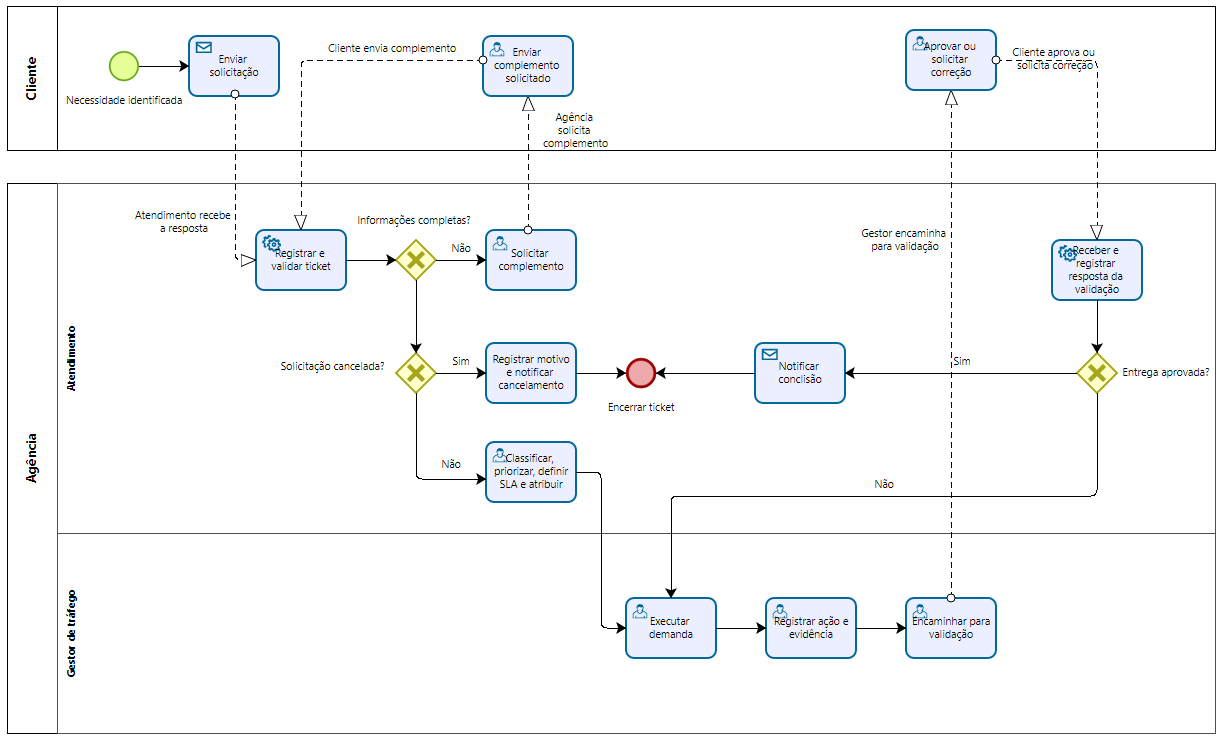
\includegraphics[width=\textwidth]{figuras/bpmn-processo-to-be.png}
\caption{Processo To Be do SIGE Desk}
\label{fig:processo-to-be}
\par\footnotesize\textbf{Fonte:} Elaborado pelo grupo, com base em BPMN 2.0.2 \cite{omg2014}.
\end{figure}

\subsection{Estados, SLA e rastreabilidade}

O ciclo de vida do ticket possui os estados Aberta, Em triagem, Em execução, Aguardando cliente, Em validação, Concluída, Reaberta e Cancelada. A conclusão requer validação ou o registro de que o tipo de demanda dispensa aprovação; o cancelamento requer justificativa; e a reabertura inicia novo ciclo de resolução sem apagar o histórico anterior.

O calendário padrão de SLA considera dias úteis, das 8h às 18h, no fuso America/Sao\_Paulo, excluindo feriados e recessos configurados. A primeira resposta é o primeiro retorno efetivo registrado ao solicitante; uma confirmação automática não a satisfaz. O prazo de resolução é pausado enquanto o ticket estiver Aguardando cliente e volta a contar quando ele retornar à execução. A Tabela \ref{tab:sla} sintetiza a configuração inicial.

\begin{table}[H]
\centering
\caption{Prazos preliminares de SLA}
\label{tab:sla}
\begin{tabular}{lcc}
\hline
\textbf{Prioridade} & \textbf{Primeira resposta} & \textbf{Resolução prevista} \\
\hline
Urgente & 2 horas úteis & 8 horas úteis \\
Alta & 4 horas úteis & 16 horas úteis \\
Média & 8 horas úteis & 24 horas úteis \\
Baixa & 16 horas úteis & 40 horas úteis \\
\hline
\end{tabular}
\par\footnotesize\textbf{Fonte:} Elaborado pelo grupo.
\end{table}

Toda mudança de status, responsável, prioridade, prazo ou aprovação deverá registrar usuário, data e hora, motivo, valor anterior e novo valor. Esse histórico, associado a comentários, anexos e evidências, sustenta a rastreabilidade e a auditoria da demanda.

\subsection{Requisitos prioritários}

Os requisitos foram organizados conforme a ISO/IEC/IEEE 29148 \cite{iso29148}. Para a primeira versão, são prioritários autenticação e autorização por perfil; cadastro de clientes e campanhas; abertura e identificação única do ticket; triagem e atribuição; atualização de status; comentários e anexos; histórico auditável; notificações; filtros; configuração de tipos de demanda e de SLA. Requisitos de segurança, privacidade, integridade, desempenho, acessibilidade, backup e retenção complementam o escopo. A matriz detalhada de requisitos e os cenários de teste estão apresentados nos Apêndices A e B.

\section{CONSIDERAÇÕES FINAIS}

O SIGE Desk foi proposto para transformar comunicações dispersas em um fluxo de atendimento rastreável, com responsáveis, prazos, validações e evidências. A solução combina fundamentos de gestão de serviços, marketing digital, gestão de projetos e proteção de dados para responder ao problema de centralização das demandas de tráfego pago.

O trabalho encontra-se na fase de especificação e prototipação. A continuidade prevê validar os requisitos com potenciais usuários, implementar o MVP, executar os casos de teste e registrar os resultados da avaliação de usabilidade. Esses resultados permitirão ajustar o processo, os requisitos e a interface antes de uma eventual adoção em contexto real.

\appendix
\section{MATRIZ SINTÉTICA DE REQUISITOS}

\begin{longtable}{p{0.16\textwidth}p{0.57\textwidth}p{0.13\textwidth}}
\caption{Requisitos funcionais prioritários}\label{tab:requisitos}\\
\hline
\textbf{ID} & \textbf{Requisito} & \textbf{Prioridade} \\
\hline
\endfirsthead
\hline
\textbf{ID} & \textbf{Requisito} & \textbf{Prioridade} \\
\hline
\endhead
RF-01/RF-02 & Autenticar usuários e restringir funções e tickets conforme perfil. & Alta \\
RF-03/RF-04 & Manter clientes ativos e campanhas vinculadas ao respectivo cliente. & Alta \\
RF-05/RF-06 & Abrir ticket com dados mínimos e gerar identificador único. & Alta \\
RF-07/RF-09 & Classificar, atribuir e auditar mudanças de prioridade, prazo, responsável e status. & Alta \\
RF-08/RF-10/RF-12 & Atualizar status, registrar comentários, anexos, ação executada e evidências. & Alta \\
RF-14/RF-17 & Filtrar tickets e consultar o histórico completo. & Alta \\
RF-20/RF-21 & Notificar envolvidos autorizados e exibir os prazos de SLA. & Alta \\
RF-22/RF-23 & Configurar tipos de demanda, campos obrigatórios, aprovações, evidências e calendário de SLA. & Alta \\
RF-11/RF-13/RF-15/RF-16 & Registrar aprovação, cancelamento, indicadores do painel e situações de vencimento. & Média \\
RF-18/RF-19 & Registrar métricas de contexto e exportar lista filtrada de tickets. & Baixa \\
\hline
\multicolumn{3}{l}{\footnotesize\textbf{Fonte:} Elaborado pelo grupo a partir dos requisitos preliminares.}
\end{longtable}

\begin{longtable}{p{0.16\textwidth}p{0.70\textwidth}}
\caption{Requisitos não funcionais}\label{tab:requisitos-nao-funcionais}\\
\hline
\textbf{Aspecto} & \textbf{Critério inicial} \\
\hline
\endfirsthead
\hline
\textbf{Aspecto} & \textbf{Critério inicial} \\
\hline
\endhead
Usabilidade & Ao menos 80\% das tarefas concluídas sem ajuda e nenhuma abaixo de 70\% de conclusão. \\
Segurança e privacidade & Senhas protegidas, autorização por perfil, auditoria de acessos e coleta apenas de dados necessários. \\
Rastreabilidade e integridade & Histórico preservado; tickets concluídos ou cancelados não podem ser apagados sem registro administrativo. \\
Desempenho & Em base de teste com 100 tickets, 90\% das operações de abertura e listagem devem concluir em até dois segundos. \\
Disponibilidade e acessibilidade & Salvamento sem perda de dados, compatibilidade com navegadores modernos, rótulos claros, contraste adequado e navegação por teclado. \\
Continuidade & Backup diário com retenção mínima de 30 dias e teste periódico de restauração; retenção de tickets e anexos por 24 meses, sujeita à revisão jurídica. \\
\hline
\multicolumn{2}{l}{\footnotesize\textbf{Fonte:} Elaborado pelo grupo a partir dos requisitos preliminares.}
\end{longtable}

\section{PLANO DE VALIDAÇÃO}

\begin{longtable}{p{0.15\textwidth}p{0.46\textwidth}p{0.25\textwidth}}
\caption{Cenários mínimos de teste funcional}\label{tab:testes}\\
\hline
\textbf{ID} & \textbf{Cenário} & \textbf{Resultado esperado} \\
\hline
\endfirsthead
\hline
\textbf{ID} & \textbf{Cenário} & \textbf{Resultado esperado} \\
\hline
\endhead
CT-01 & Cliente abre ticket de alteração de campanha. & Ticket recebe identificador, status inicial, urgência e prazo desejado. \\
CT-02 & Atendimento classifica e atribui o ticket. & Prioridade, SLA e responsável ficam registrados; confirmação automática não conta como primeira resposta. \\
CT-03 a CT-05 & Responsável atualiza o ticket, solicita informação, valida e trata correção. & Histórico, evidência, estados de aguardo e validação, aprovação ou reabertura são preservados. \\
CT-06 e CT-07 & Usuário consulta demandas vencidas e acompanha eventos. & Filtros retornam os tickets corretos e envolvidos recebem notificação configurada. \\
CT-08 e CT-09 & Cliente tenta acesso indevido e administrador restaura backup de teste. & Acesso é negado e registrado; dados e anexos são recuperados conforme a política. \\
CT-10 & Usuário abre e lista tickets em base com 100 registros. & Pelo menos 90\% das operações concluem em até dois segundos. \\
CT-11 a CT-15 & Administrador configura tipo, SLA e cadastros; usuário consulta auditoria. & Regras configuradas são aplicadas e o histórico exibe autor, data, motivo e valores alterados. \\
\hline
\multicolumn{3}{l}{\footnotesize\textbf{Fonte:} Elaborado pelo grupo a partir do plano de testes preliminar.}
\end{longtable}
